\begin{figure}[H]
    \centering
    \begin{subfigure}[t]{.49\textwidth}
        \centering
        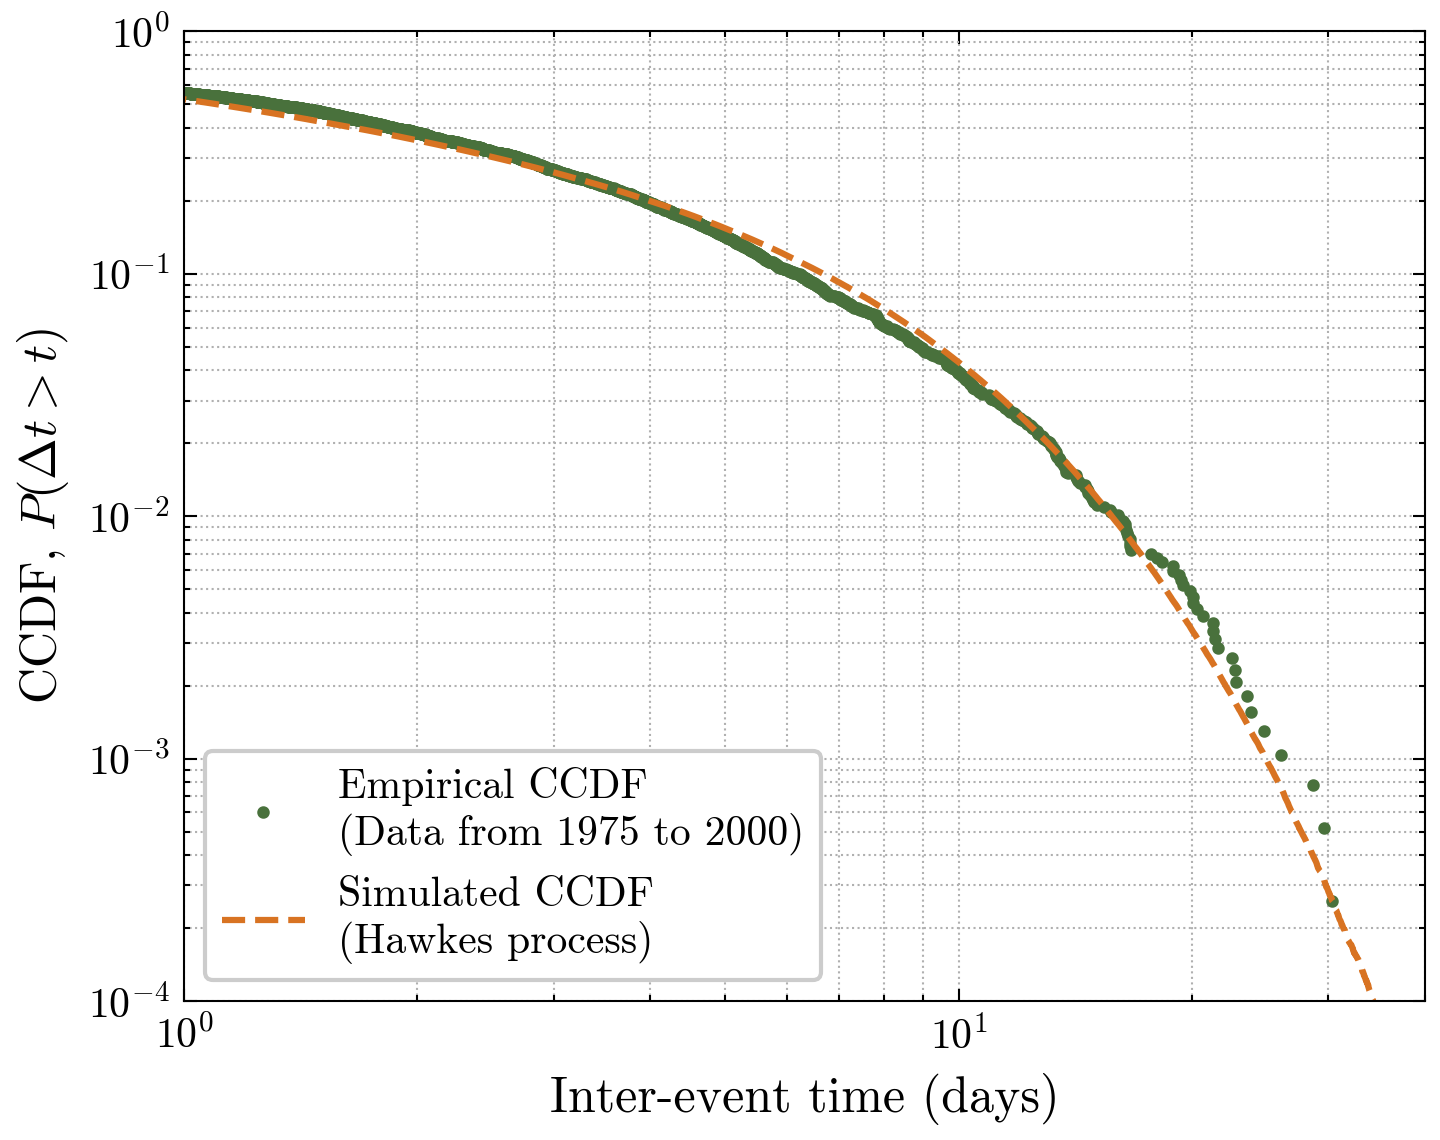
\includegraphics[width=\textwidth]{figures/hawkes-ccdf.png}
        \caption{CCDF of inter-event times in log-log scale}
        \label{fig:hawkes-ccdf}
    \end{subfigure}%
    \hspace{1em}
    \begin{subfigure}[t]{.47\textwidth}
        \centering
        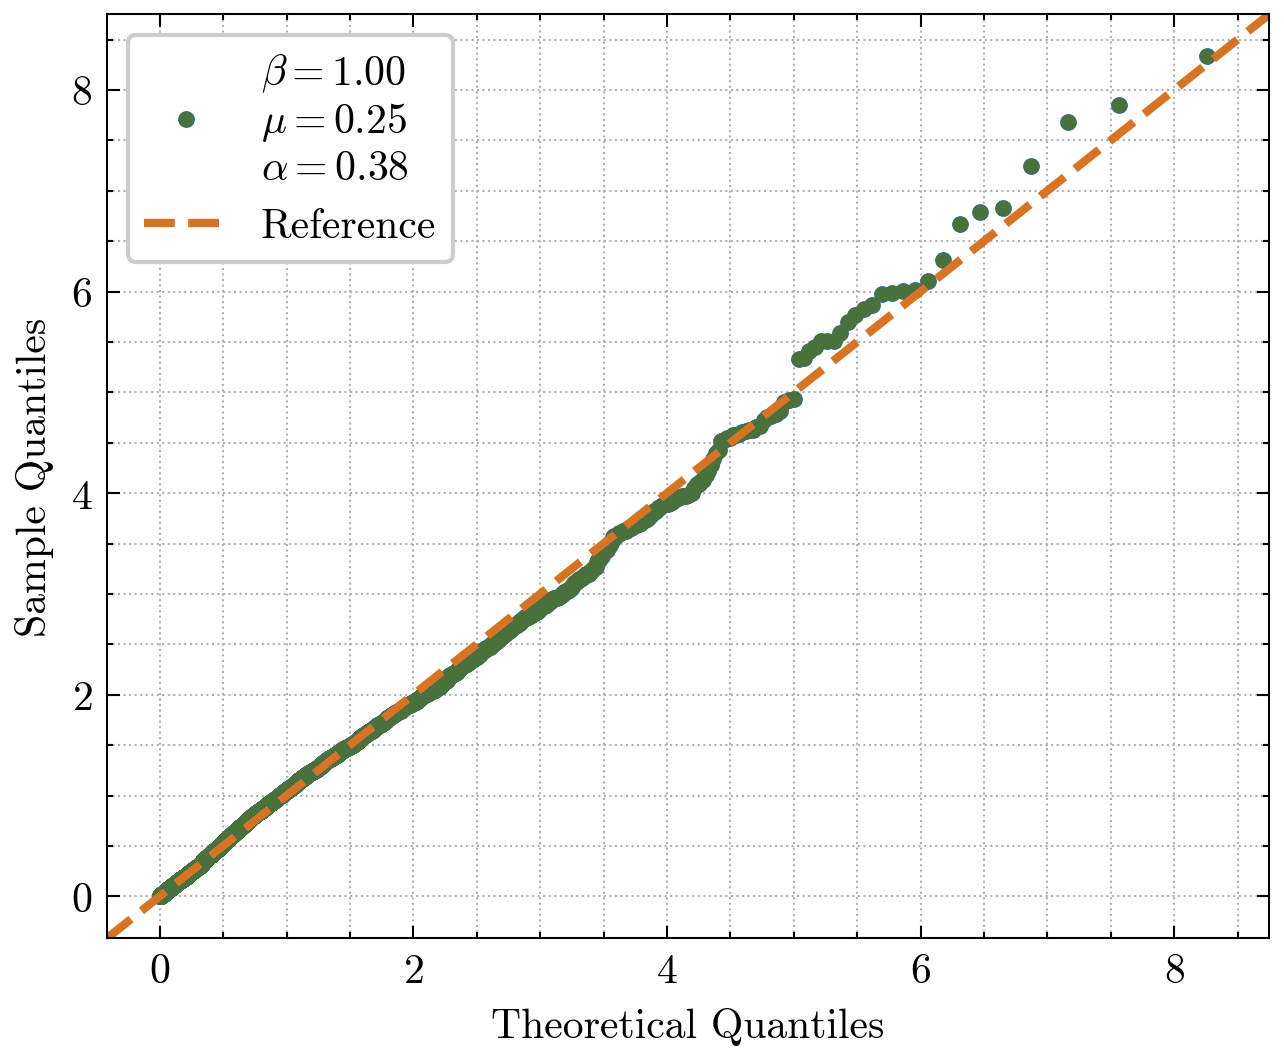
\includegraphics[width=\textwidth]{figures/hawkes-qq.png}
        \caption{QQ plot of inter-event times transformed via time-rescaling theorem with the fitted Hawkes model}
        \label{fig:hawkes-qq}
    \end{subfigure}
    \caption{Simulated vs empirical inter-event times for the fitted Hawkes model on murders in Sicily (1975-2000). The good agreement indicates a good fit of the model to the data.}
\end{figure}